\documentclass[12pt]{report}

\usepackage{amsmath,amsfonts,amssymb,amsthm} % AMS Family
\usepackage[utf8]{inputenc}
\usepackage[english]{babel}
\usepackage{enumerate}
\usepackage[Glenn]{fncychap}% for the chapter header style
% \usepackage{fontspec}
\usepackage{fullpage}
\usepackage{mathtools}% for xRightarrow
\usepackage{nicefrac}% for some inline fraction styles
\usepackage{enumitem}% for enumerate and itemize
\usepackage{tikz}
\usepackage{libertine}
\usepackage[T1]{fontenc}
\usepackage{inconsolata}
\usepackage{url}

\usetikzlibrary{automata}
\usetikzlibrary{trees}
\usetikzlibrary{positioning}

\setcounter{chapter}{-2}

\newcommand{\dfa}{\textsf{DFA}}
\newcommand{\nfa}{\textsf{NFA}}
\newcommand{\cfg}{\textsf{CFG}}
\newcommand{\cfl}{\textsf{CFL}}
\newcommand{\pda}{\textsf{PDA}}
\newcommand{\emptystring}{$\varepsilon$}
\newcommand{\derivation}{\xRightarrow{\ast}}

\begin{document}

\title{Solutions to \emph{Introduction to the Theory of Computation, Third Edition}}
\author{Cheng Luyu}
\date{April 2017}
\maketitle

\tableofcontents

\chapter{Before the Solutions}

\chapter{Introduction}

To be done.

\part{Automata and Languages}

\chapter{Regular Languages}

\section*{Exercises}

\begin{enumerate}[font=\bfseries]

    \item The following are the state diagrams of two \dfa s, $M_1$ and $M_2$ . Answer the following questions about each of these machines.
    
    \begin{enumerate}[font=\bfseries,label=\alph*.]
        \item What is the start state?
        \item What is the set of accept states?
        \item What sequence of states does the machine go through on input {\tt aabb}?
        \item Does the machine accept the string {\tt aabb}?
        \item Does the machine accept the string \emptystring?
    \end{enumerate}
    
    \item Give the formal description of the machines $M_1$ and $M_2$ pictured in Exercise 1.1.
    
    \item[2.4]
    \begin{enumerate}[font=\bfseries]
        \item[c.]
        \item[e.]
    \end{enumerate}
    
    \item[2.6]
    \begin{enumerate}[font=\bfseries]
        \item[b.]
        \item[d.]
    \end{enumerate}

\end{enumerate}

\section*{Problems}

\begin{enumerate}

    \item[{\bf 1.29b}]
    
    Assume that $A_2=\{www|w\in\{\texttt{a},\texttt{b}\}^\ast\}$ is regular. Let $p$ be the pumping length given by the pumping lemma. Choose $s$ to be the string $\texttt{a}^p\texttt{ba}^p\texttt{ba}^p\texttt{b}$. Because $s$ is a member of $A_2$ and $s$ is longer than $p$, the pumping lemma guarantees that $s$ can be split into three pieces, $s=xyz$, satisfying the three conditions of the pumping lemma. According to condition 3, $y$ must consists only of {\tt a}s. Hence $xyyz$ is not a member of $A_2$, a contradiction. Therefore $A_2$ is not regular.
    
    \item[{\bf 1.30}]
    
    The proof is wrong because we cannot conclude a contradiction from Example 1.73. Re-consider cases.
    
    \begin{enumerate}
    \item The string $y$ consists only of {\tt 0}s. In this case, the string $xyyz$ is a member of $B$. This case is not a contradiction.
    \item The string $y$ consists only of {\tt 1}s. This case is also not a contradiction.
    \end{enumerate}
    
    None of them are contradiction, where error lies.
    
    \item[{\bf 1.46d}]
    
    We will use a proof by contradiction. Assume that $L$ is a regular language. Then by the pumping lemma, there exists a pumping length $p$ for $L$ such that for any string $s\in L$ where $|s|\ge p$, $s=xyz$ subject to the following conditions:
    
    \begin{enumerate}
    \item[1.] $|y| > 0$,
    \item[2.] $|xy|\le p$, and
    \item[3.] for all $i>0,xy^iz\in L$.
    \end{enumerate}
    
    Choose $s={\tt 0}^p{\tt 110}^p{\tt 1}$. Clearly $s\in L$ with $w={\tt 0}^p{\tt 1}$ and $t={\tt 1}$, and $|s|\ge p$. By the second condition of pumping lemma, it is obvious that $xy$ consists only of zeros, and further, by first condition and second condition, it follows that $y = 0^k$ for some $k > 0$. By the third condition, we can take any $i$ and $xy^iz$ will be in $L$. Taking $i = 2$, then $xyyz\in L$. $xyyz = xyyz = {\tt 0}^{(p+k)}{\tt 110}^p{\tt 1}$. There is no way that this string can be divided into $wtw$ as required to be in $L$, thus $xyyz\notin L$, a contradiction. Therefore $L$ is not a regular language.
    
    \item[{\bf 1.53}]
    
    Assume that $ADD$ is regular. Let $p$ be the pumping length given by the pumping lemma. Choose $s$ to be the string ${\tt 1}^p${\tt =}${\tt 1}^{p-1}${\tt 0+1}. Because $s$ is a member of $ADD$ and $s$ is longer than $p$, the pumping lemma guarantees that $s$ can be split into three pieces, $s=xyz$, satisfying the three conditions of the pumping lemma. Thus $y$ must consists of only {\tt 1}s. Let $y={\tt 1}^k$ where $0<k\le p$. Since $xyyz={\tt 1}^{p+k}${\tt =}${\tt 1}^{p-1}${\tt 0+1}$\notin ADD$, a contradiction. Therefore $ADD$ is not regular.
    
    \item[{\bf 1.54}]
    \begin{enumerate}
        \item[{\bf a.}] We claim all strings of the form $ab^i$ must be in distinct equivalence classes for all $i\ge 0$. This is because any two strings $ab^{i_1}$ and $ab^{i_2}$ can be distinguished by $c^{i_1}$, since $ab^{i_1}c^{i_1}\in F$, while $ab^{i_2}c^{i_1} \notin F$. Since there are infinitely many equivalence classes of the indistinguishability relation, we conclude by the Myhill-Nerode theorem, which is claimed in Problem 1.52, that no DFA can recognize $F$.
        
        \item[{\bf b.}] The pumping lemma says that for any string $s$ in the language, with length greater than the pumping length $p$, we can write $s = xyz$ with $|xy|\le p$, such that $xy^iz$ is also in the language for every $i\ge 0$.
        
        For the given language, we can take $p = 2$. Consider any string ${\tt a}^i{\tt b}^j{\tt c}^k$ in the language. If $i=1$ or $i>2$ ,we take $x=\varepsilon$ and $y={\tt a}$. If $i=1$, we must have $j=k$ and adding any number of a’s still preserves the membership in the language. For $i > 2$, all strings obtained by pumping $y$ as defined above, have two or more \texttt{a}’s and hence are always in the language.
        
        For $i = 2$, we can take $x = \varepsilon$ and $y = {\tt aa}$. Since the strings obtained by pumping in this case always have an even number of \texttt{a}’s, they are all in the language. Finally, for the case $i=0$, we take $x=\varepsilon$, and $y={\tt b}$ if $j>0$ and $y={\tt c}$ otherwise. Since strings of the form ${\tt b}^j{\tt c}^k$ are always in the language, we satisfy the conditions of the pumping lemma in this case as well.
        
        \item[{\bf c.}] Because the pumping lemma only says that if a language is regular, then it must satisfy the conditions of the lemma. However, this does not necessarily mean that no non-regular language can satisfy these conditions.
    \end{enumerate}
    
    \item[{\bf 1.55}]
    \begin{enumerate}
        \item[{\bf f.}] The minimum pumping length is 1. The only member in the language is $\varepsilon$, which cannot be pumped. It cannot be 0 because the third condition of pumping lemma requires $|y|>0$.
        \item[{\bf g.}]
        
        The minimum pumping length is 3. The string {\tt 00} is in the language but cannot be pumped, so 2 is not a pumping length for this language. If $s$ has length 3 or more, it must contains 1s. By dividing $s$ into $xyz$, where $x$ is everything in front of the first {\tt 1} and $y$ is the first {\tt 1} and $z$ is everything afterward, we satisfy the pumping lemma’s three conditions.
        
        \item[{\bf h.}]
        
        The minimum pumping length is 4. The string {\tt 100} is in the language but cannot be pumped, so 3 is not a pumping length for this language. If $s$ has length 4 or more, it must contains at least two 1s. By dividing $s$ into $xyz$, where $x$ is {\tt 10} and $y$ is the second {\tt 1} and $z$ is everything afterward, we satisfy the pumping lemma’s three conditions.
        
        \item[{\bf i.}]
        
        The minimum pumping length is 5. The sole string {\tt 1011} in the language cannot be pumped, so 4 is not a pumping length for this language. Thus the minimum pumping length is $4+1=5$.
        
        \item[{\bf j.}]
        
        The minimum pumping length is 1. The empty string $\varepsilon$ is in the language but cannot be pumped. Choose $s$ where $|s|>0$ from $\Sigma^\ast$ randomly. It can be divided into $xyz$, where $x$ is $\varepsilon$ and $y$ is the first symbol in $s$ and $z$ is everything afterward, we satisfy the pumping lemma's three conditions.
    \end{enumerate}
    
    \item[{\bf Extra}] Prove that the language of arithmetic expressions, which consist of {\tt +},{\tt -},$\times$,$\div$,{\tt (},{\tt )} and positive integers composed of non-zero digits, are not regular.
    
    Let $L$ be the language. Assume that $L$ is regular. Let $p$ be the pumping length given by the pumping lemma. Choose $s$ to be the string {\tt (}$^p${\tt 1)}$^p$. Because $s$ is a member of $L$ and $s$ is longer than $p$, the pumping lemma guarantees that $s$ can be split into three pieces, $s=xyz$, satisfying the three conditions of the pumping lemma. Thus $y$ must consists of only {\tt (}s. Let $y=${\tt (}$^k$ where $0<k\le p$. Since $xyyz=${\tt (}$^{p+k}${\tt 1)}$^p\notin ADD$, a contradiction. Therefore $L$ is not regular.

\end{enumerate}

\chapter{Context-Free Language}

\section*{Solutions to Exercises}

\begin{enumerate}[font=\bfseries,label=2.\arabic*]

%%%%%%%%%%%%%%%%%%%%%%%%%%%%%%%%% Exercise 2.1 %%%%%%%%%%%%%%%%%%%%%%%%%%%%%%%%

\item Recall the \cfg ~$G_4$ that we gave in Example 2.4. For convenience, let’s rename its variables with single letters as follows.

\begin{align*}
    E &\rightarrow E {\tt +} T \mid T \\
    T &\rightarrow T \texttt{$\times$} F \mid F \\
    F &\rightarrow (E) \mid {\tt a} \\
\end{align*}

Give parse trees and derivations for each string.

\begin{enumerate}[font=\bfseries,label=\alph*.]

    %%%%%%%%%%%%%%%%%%%%%%%%%% Exercise 2.2.a %%%%%%%%%%%%%%%%%%%%%%%%%
    \item {\tt a}
    
    Solution: The derivations is $$E\Rightarrow T\Rightarrow F\Rightarrow \texttt{a}$$ and the parse trees is given in Figure \ref{ex-2-1-a}.
    
    \begin{figure}
    \centering
    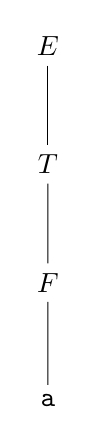
\begin{tikzpicture}[
      tlabel/.style={pos=0.4,right=-1pt,font=\footnotesize\color{red!70!black}},
    ]   
        \node{$E$}
        child {
            node {$T$}
            child {
                node {$F$}
                child {
                    node {\tt a}
                }
            }
        };
    \end{tikzpicture}
    \caption{The parse tree of Exercise 2.1.a.}
    \label{ex-2-1-a}
    \end{figure}
    
    %%%%%%%%%%%%%%%%%%%%%%%%%% Exercise 2.2.b %%%%%%%%%%%%%%%%%%%%%%%%%
    \item {\tt a+a}
    
    Solution: The derivations (left-most) is $$E\Rightarrow E+T\Rightarrow T+T\Rightarrow F+T\Rightarrow F+F\Rightarrow {\tt a}+F\Rightarrow {\tt a}+{\tt a}$$ and the parse trees is given in Figure \ref{ex-2-1-b}.
    
    \begin{figure}
    \centering
    \begin{tikzpicture}[
      tlabel/.style={pos=0.4,right=-1pt,font=\footnotesize\color{red!70!black}},
    ]   
        \node{$E$}
        child {
            node {$E$}
            child {
                node {$T$}
                child {
                    node {$F$}
                    child {
                        node {\tt a}
                    }
                }
            }
        }
        child { node {\tt +} }
        child {
            node {$T$}
            child {
                node {$F$}
                child {
                    node {\tt a}
                }
            }
        };
    \end{tikzpicture}
    \caption{The parse tree of Exercise 2.1.b.}
    \label{ex-2-1-b}
    \end{figure}
    
    %%%%%%%%%%%%%%%%%%%%%%%%%% Exercise 2.2.c %%%%%%%%%%%%%%%%%%%%%%%%%
    \item {\tt a+a+a}
    
    Solution: The derivations (left-most) is 
    \begin{align*}
        E &\Rightarrow E+T\Rightarrow E+T+T\Rightarrow T+T+T\Rightarrow F+T+T\Rightarrow F+F+T\\
        &\Rightarrow F+F+F\Rightarrow {\tt a}+F+F\Rightarrow {\tt a}+{\tt a}+F\Rightarrow {\tt a}+{\tt a}+{\tt a}
    \end{align*}    
    and the parse trees is given in Figure \ref{ex-2-1-c}.
    
    \begin{figure}
    \centering
    \begin{tikzpicture}[
      tlabel/.style={pos=0.4,right=-1pt,font=\footnotesize\color{red!70!black}},
    ]   
        \node{$E$}
        child {
            node {$E$}
            child {
                node {$E$}
                child {
                    node {$T$}
                    child {
                        node {$F$}
                        child {
                            node {\tt a}
                        }
                    }
                }
            }
            child { node {\tt +} }
            child {
                node {$T$}
                child {
                    node {$F$}
                    child {
                        node {\tt a}
                    }
                }
            }
        }
        child { node {\tt +} }
        child {
            node {$T$}
            child {
                node {$F$}
                child {
                    node {\tt a}
                }
            }
        };
    \end{tikzpicture}
    \caption{The parse tree of Exercise 2.1.c.}
    \label{ex-2-1-c}
    \end{figure}
    
    %%%%%%%%%%%%%%%%%%%%%%%%%% Exercise 2.2.d %%%%%%%%%%%%%%%%%%%%%%%%%
    \item {\tt ((a))}
    
    Solution: The derivations (left-most) is $$E\Rightarrow T\Rightarrow F\Rightarrow (E)\Rightarrow (T)\Rightarrow (F)\Rightarrow ((E))\Rightarrow ((T))\Rightarrow ((F))\Rightarrow (({\tt a}))$$ and the parse trees is given in Figure \ref{ex-2-1-d}.
    
    \begin{figure}
    \centering
    \begin{tikzpicture}[
      tlabel/.style={pos=0.4,right=-1pt,font=\footnotesize\color{red!70!black}},
    ]   
        \node{$E$}
        child {
            node {\tt (}
        }
        child {
            node {$E$}
            child {
                node {\tt (}
            }
            child {
                node{$E$}
                child {
                    node {$T$}
                    child {
                        node {$F$}
                        child {
                            node {\tt a}
                        }
                    }
                }
            }
            child {
                node {\tt )}
            }
        }
        child {
            node {\tt )}
        };
    \end{tikzpicture}
    \caption{The parse tree of Exercise 2.1.d.}
    \label{ex-2-1-d}
    \end{figure}
\end{enumerate}

%%%%%%%%%%%%%%%%%%%%%%%%%%%%%%%%% Exercise 2.2 %%%%%%%%%%%%%%%%%%%%%%%%%%%%%%%%

\item

\begin{enumerate}[font=\bfseries,label=\alph*.]
    \item Use the languages $A = \{{\tt a}^m {\tt b}^n {\tt c}^n | m, n\ge 0\}$ and $B = \{{\tt a}^n {\tt b}^n {\tt c}^m | m, n\ge 0\}$ together with Example 2.36 to show that the class of context-free languages is not closed under intersection.

    \item Use part (a) and DeMorgan’s law (Theorem 0.20) to show that the class of context-free languages is not closed under complementation.
\end{enumerate}

%%%%%%%%%%%%%%%%%%%%%%%%%%%%%%%%% Exercise 2.3 %%%%%%%%%%%%%%%%%%%%%%%%%%%%%%%%

\item

Answer each part for the following context-free grammar $G$. 
\begin{align*}
R &\rightarrow XRX \mid S\\
S &\rightarrow {\tt a} T {\tt b} \mid {\tt b} T {\tt a}\\
T &\rightarrow XTX \mid X \mid \varepsilon\\
X &\rightarrow {\tt a} \mid {\tt b}
\end{align*}

\begin{enumerate}[font=\bfseries,label=\alph*.]
    \item What are the variables of $G$?
    
    Answer: $V=\{R,S,T,X\}$
    
    \item What are the terminals of $G$? 
    
    Answer: $\Sigma=\{{\tt a},{\tt b}\}$
    
    \item Which is the start variable of $G$? 
    
    Answer: The start variable is $R$.
    
    \item Give three strings in $L(G)$. 
    
    Answer: {\tt ab}, {\tt ba} and {\tt aabb}.
    
    \item Give three strings not in $L(G)$.
    
    Answer: {\tt aa}, {\tt aaa} and {\tt aaaa}.
    
    \item True or False: $T\Rightarrow {\tt aba}$.
    
    Answer: False.
    
    \item True or False: $T\derivation {\tt aba}$.
    
    Answer: True. In the following derivations: $$T\Rightarrow XTX\Rightarrow {\tt a}TX\Rightarrow {\tt a}XX\Rightarrow {\tt a}{\tt b}X\Rightarrow {\tt a}{\tt b}{\tt a}$$
    
    \item True or False: $T\Rightarrow T$.
    
    Answer: False.
    
    \item True or False: $T\derivation T $.
    
    Answer: False.
    
    \item True or False: $XXX\derivation {\tt aba}$.
    
    Answer: True. In the following derivations: $$XXX\Rightarrow {\tt a}XX\Rightarrow {\tt a}{\tt b}X\Rightarrow {\tt a}{\tt b}{\tt a}$$
    
    \item True or False: $X\derivation {\tt aba}$.
    
    Answer: False.
    
    \item True or False: $T\derivation XX$.
    
    Answer: True. In the following derivations: $$T\Rightarrow XTX\Rightarrow X\varepsilon X=XX$$
    \item True or False: $T\derivation XXX$.
    
    Answer: True. In the following derivations: $$T\Rightarrow XTX\Rightarrow XXX$$
    \item True or False: $S\derivation \varepsilon$.
    
    Answer: False.
    \item Give a description in English of $L(G)$.
\end{enumerate}

%%%%%%%%%%%%%%%%%%%%%%%%%%%%%%%%% Exercise 2.4 %%%%%%%%%%%%%%%%%%%%%%%%%%%%%%%%

\item Give context-free grammars that generate the following languages. In all parts, the alphabet $\Sigma$ is $\{0,1\}$.

\begin{enumerate}[font=\bfseries,label=\alph*.]
    \item $\{w| w\text{ contains at least three \texttt{1}s}\}$
    \begin{align*}
        R &\rightarrow SSS \\
        S &\rightarrow T{\tt 1}T \\
        T &\rightarrow {\tt 0}T \mid {\tt 1}T \mid \varepsilon
    \end{align*}
    
    \item $\{w| w\text{ starts and ends with the same symbol}\}$
    \begin{align*}
        R &\rightarrow {\tt 0}S{\tt 0} \mid {\tt 1}S{\tt 1} \\
        S &\rightarrow {\tt 0}S \mid {\tt 1}S \mid \varepsilon
    \end{align*}
    
    \item $\{w| \text{the length of $w$ is odd}\}$
    \begin{align*}
        R &\rightarrow {\tt 1}S \mid {\tt 0}S \\
        S &\rightarrow {\tt 00} \mid {\tt 01} \mid {\tt 10} \mid {\tt 11} \mid \varepsilon
    \end{align*}
    
    \item $\{w| \text{the length of $w$ is odd and its middle symbol is a 0}\}$
    \begin{align*}
        R &\rightarrow S{\tt 0}S \\
        S &\rightarrow {\tt 00} \mid {\tt 01} \mid {\tt 10} \mid {\tt 11} \mid \varepsilon
    \end{align*}
    
    
    \item $\{w| w = w^\mathcal R, \text{that is,$w$ is a palindrome}\}$
    \begin{align*}
        R &\rightarrow {\tt 0}R{\tt 0} \mid {\tt 1}R{\tt 1} \mid \varepsilon
    \end{align*}
    
    \item The empty set
    \begin{align*}
        R &\rightarrow R
    \end{align*}

\end{enumerate}

%%%%%%%%%%%%%%%%%%%%%%%%%%%%%%%%% Exercise 2.5 %%%%%%%%%%%%%%%%%%%%%%%%%%%%%%%%

\item Give informal descriptions and state diagrams of pushdown automata for the languages in Exercise 2.4.


\begin{enumerate}[font=\bfseries,label=\alph*.]
    \item $\{w| w\text{ contains at least three \texttt{1}s}\}$
    
    \item $\{w| w\text{ starts and ends with the same symbol}\}$
    
    \begin{figure}
    \centering
    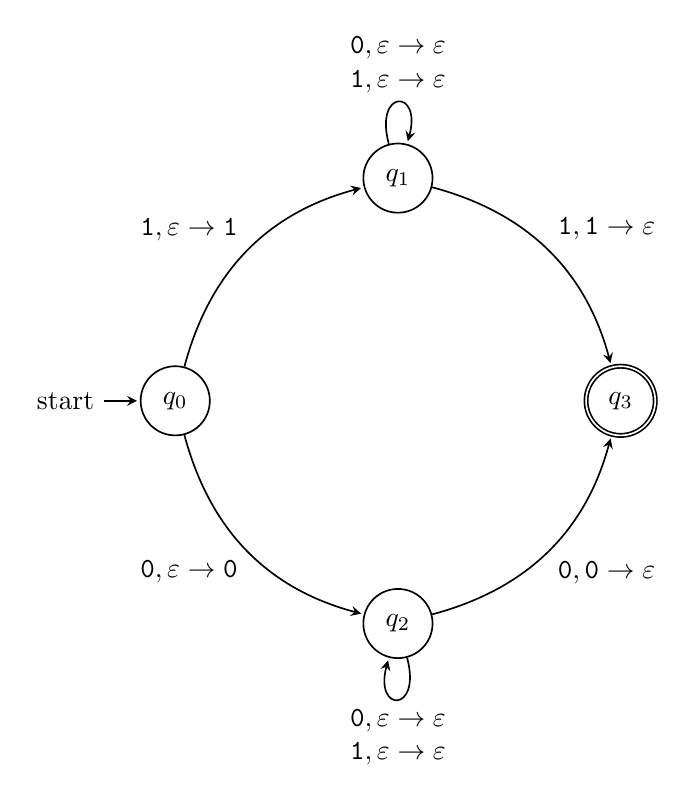
\begin{tikzpicture}[->,>=stealth,semithick,shorten >=1pt,node distance=4cm,on grid,auto] 
        \node[state,initial] (q0) {$q_0$};
        \node[state] (q1) [above right=of q0] {$q_1$};
        \node[state] (q2) [below right=of q0] {$q_2$};
        \node[state,accepting] (q3) [below right=of q1] {$q_3$};
        \path   (q0) edge [bend left] node {$\texttt{1},\varepsilon\rightarrow\texttt{1}$} (q1)
                     edge [bend right] node [below left] {$\texttt{0},\varepsilon\rightarrow\texttt{0}$} (q2)
                (q1) edge [bend left] node {$\texttt{1},\texttt{1}\rightarrow\varepsilon$} (q3)
                     edge [loop above] node[align=center] {$\texttt{0},\varepsilon\rightarrow\varepsilon$\\$ \texttt{1},\varepsilon\rightarrow\varepsilon$} (q1)
                (q2) edge [bend right] node [below right] {$\texttt{0},\texttt{0}\rightarrow\varepsilon$} (q3)
                     edge [loop below] node[align=center] {$\texttt{0},\varepsilon\rightarrow\varepsilon$\\$\texttt{1},\varepsilon\rightarrow\varepsilon$} (q2);
    \end{tikzpicture}
    \caption{A possible solution to exercise 2.5}
    \end{figure}

    \item $\{w| \text{the length of $w$ is odd}\}$
    
    \item $\{w| \text{the length of $w$ is odd and its middle symbol is a 0}\}$
    
    \item $\{w| w = w^\mathcal R, \text{that is,$w$ is a palindrome}\}$
    
    \begin{figure}
    \centering
    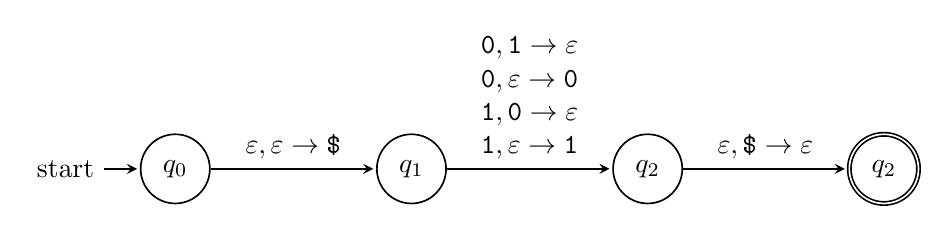
\begin{tikzpicture}[->,>=stealth,semithick,shorten >=1pt,node distance=3cm,on grid,auto] 
        \node[state,initial] (q0) {$q_0$};
        \node[state] (q1) [right=of q0] {$q_1$};
        \node[state] (q2) [right=of q1] {$q_2$};
        \node[state,accepting] (q3) [right=of q2] {$q_2$};
        \path   (q0) edge node {$\varepsilon,\varepsilon\rightarrow\texttt{\$}$} (q1)
                (q1) edge node[align=center] {$\texttt{0},\texttt{1}\rightarrow\varepsilon$\\
                                $\texttt{0},\varepsilon\rightarrow\texttt{0}$\\
                                $\texttt{1},\texttt{0}\rightarrow\varepsilon$\\
                                $\texttt{1},\varepsilon\rightarrow\texttt{1}$} (q2)
                (q2) edge node {$\varepsilon,\texttt{\$}\rightarrow\varepsilon$} (q3);
    \end{tikzpicture}
    \caption{A possible solution to exercise 2.5}
    \end{figure}
    
    \item The empty set
\end{enumerate}

%%%%%%%%%%%%%%%%%%%%%%%%%%%%%%%%% Exercise 2.6 %%%%%%%%%%%%%%%%%%%%%%%%%%%%%%%%

\item Give context-free grammars generating the following languages.

\begin{enumerate}[font=\bfseries,label=\alph*.]
    \item The set of strings over the alphabet $\{{\tt a},{\tt b}\}$ with more {\tt a}’s than {\tt b}’s
    
    \emph{Answer}
    \begin{align*}
        A\rightarrow B
    \end{align*}
    
    \item The complement of the language $\{{\tt a}^n {\tt b}^n | n \ge 0\}$
    
    \emph{Answer}:
    \begin{equation*}
    \begin{split}
        R &\rightarrow S \mid V \mid W \\
        S &\rightarrow {\tt a}S{\tt a} \mid {\tt b}S{\tt b} \mid \varepsilon \\
        T &\rightarrow {\tt a}T \mid \varepsilon \\
        U &\rightarrow {\tt b}T \mid \varepsilon \\
        V &\rightarrow {\tt b}X \\
        W &\rightarrow {\tt a}T{\tt b}U{\tt a}X \\
        X &\rightarrow {\tt a}X \mid {\tt b}X \mid \varepsilon
    \end{split}
    \end{equation*}
    
    \item $\left\{w{\tt \#}x| w^\mathcal R \text{ is a substring of $x$ for } w, x\in \{0,1\}^\ast \right\}$
    
    \item $\left\{x_1{\tt \#}x_2{\tt \#}\cdots{\tt \#}x_k | k\ge 1, \text{ each } x_i \in \{a, b\}^\ast , \text{and for some $i$ and $j$}, x_i = x_j^\mathcal R \right\}$
    
    \emph{Answer}:
    \begin{equation*}
    \begin{split}
        R &\rightarrow SR' \\
        R'&\rightarrow {\tt \#}SR' \mid \varepsilon \\
        S &\rightarrow T \mid U \\
        T &\rightarrow {\tt a}T{\tt a} \mid {\tt b}T{\tt b} \mid {\tt \#}R{\tt \#} \mid \varepsilon \\
        U &\rightarrow {\tt a}U \mid {\tt b}U \mid \varepsilon
    \end{split}
    \end{equation*}
    
\end{enumerate}

%%%%%%%%%%%%%%%%%%%%%%%%%%%%%%%%% Exercise 2.7 %%%%%%%%%%%%%%%%%%%%%%%%%%%%%%%%

\item Give informal English descriptions of \pda s for the languages in Exercise 2.6.

%%%%%%%%%%%%%%%%%%%%%%%%%%%%%%%%% Exercise 2.8 %%%%%%%%%%%%%%%%%%%%%%%%%%%%%%%%

\item Show that the string {\tt the girl touches the boy with the flower} has two different leftmost derivations in grammar $G_2$ on page 103. Describe in English the two different meanings of this sentence.

%%%%%%%%%%%%%%%%%%%%%%%%%%%%%%%%% Exercise 2.9 %%%%%%%%%%%%%%%%%%%%%%%%%%%%%%%%

\item Give a context-free grammar that generates the language
$$A = \{{\tt a}^i {\tt b}^j {\tt c}^k | i = j \text{ or } j = k \text{ where } i, j, k\ge 0\}. $$
Is your grammar ambiguous? Why or why not?

\emph{Answer}:
\begin{align*}
    R &\rightarrow ST \mid UV \\
    S &\rightarrow {\tt a}S{\tt b} \mid \varepsilon \\
    T &\rightarrow {\tt c}T \mid \varepsilon \\
    U &\rightarrow {\tt a}U \mid \varepsilon \\
    V &\rightarrow {\tt b}V{\tt c} \mid \varepsilon
\end{align*}

The grammar is ambiguous. Take string {\tt aabbcc} for an example, there are two derivations:
\begin{align*}
    R &\Rightarrow ST\Rightarrow {\tt a}S{\tt b}T\Rightarrow {\tt aa}S{\tt bb}T
       \Rightarrow {\tt aa}\varepsilon{\tt bb}T \Rightarrow {\tt aa}\varepsilon{\tt bbc}T
       \Rightarrow {\tt aa}\varepsilon{\tt bbcc}T \Rightarrow {\tt aa}\varepsilon{\tt bbcc}\varepsilon\\
    R &\Rightarrow UV\Rightarrow {\tt a}UV\Rightarrow {\tt aa}UV
       \Rightarrow {\tt aa}\varepsilon V\Rightarrow {\tt aa}\varepsilon {\tt b}V{\tt c}
       \Rightarrow {\tt aa}\varepsilon {\tt bb}V{\tt cc}
       \Rightarrow {\tt aa}\varepsilon {\tt bb}\varepsilon {\tt cc}
\end{align*}

%%%%%%%%%%%%%%%%%%%%%%%%%%%%%%%%% Exercise 2.10 %%%%%%%%%%%%%%%%%%%%%%%%%%%%%%%%

\item Give an informal description of a pushdown automaton that recognizes the language $A$ in Exercise 2.9.

%%%%%%%%%%%%%%%%%%%%%%%%%%%%%%%%% Exercise 2.11 %%%%%%%%%%%%%%%%%%%%%%%%%%%%%%%%

\item Convert the \cfg~$G_4$ given in Exercise 2.1 to an equivalent \pda, using the procedure given in Theorem 2.20.

%%%%%%%%%%%%%%%%%%%%%%%%%%%%%%%%% Exercise 2.12 %%%%%%%%%%%%%%%%%%%%%%%%%%%%%%%%

\item Convert the \cfg~$G$ given in Exercise 2.3 to an equivalent \pda, using the procedure given in Theorem 2.20.

%%%%%%%%%%%%%%%%%%%%%%%%%%%%%%%%% Exercise 2.13 %%%%%%%%%%%%%%%%%%%%%%%%%%%%%%%%

\item Let $G = (V, \Sigma, R, S)$ be the following grammar. $V = \{S, T, U\}$; $\Sigma = \{0, {\tt \#}\}$; and $R$ is the set of rules:

\begin{align*}
S &\rightarrow TT \mid U\\
T &\rightarrow {\tt 0}T \mid T {\tt 0} \mid {\tt \#}\\
U &\rightarrow {\tt 0}U{\tt 00} \mid {\tt \#}
\end{align*}

\begin{enumerate}[font=\bfseries,label=\alph*.]
    \item Describe $L(G)$ in English.
    \item Prove that $L(G)$ is not regular.
    
    \begin{proof}
    
    Let's 
    
    \end{proof}
\end{enumerate}

%%%%%%%%%%%%%%%%%%%%%%%%%%%%%%%%% Exercise 2.14 %%%%%%%%%%%%%%%%%%%%%%%%%%%%%%%%

\item Convert the following \cfg~into an equivalent \cfg~in Chomsky normal form, using the procedure given in Theorem 2.9.

\begin{align*}
A &\rightarrow BAB \mid B \mid \varepsilon\\
B &\rightarrow {\tt 00} \mid \varepsilon
\end{align*}

\emph{Solution}: At the first stage, we add a new start variable $S$ and the rule $S\rightarrow A$.
\begin{equation*}
\begin{split}
    \boldsymbol{S} &\boldsymbol{\rightarrow A}\\
    A &\rightarrow BAB \mid B \mid \varepsilon\\
    B &\rightarrow {\tt 00} \mid \varepsilon
\end{split}
\end{equation*}

At the second stage. First we need to remove a $\varepsilon$-rule of $B$, and add a new rule $A\rightarrow A$ and $A\rightarrow\varepsilon$. Then remove the $\varepsilon$-rules of $A$, i.e. $A\rightarrow A$ and $A\rightarrow\varepsilon$. 

%%%%%%%%%%%%%%%%%%%%%%%%%%%%%%%%% Exercise 2.15 %%%%%%%%%%%%%%%%%%%%%%%%%%%%%%%%

\item Give a counterexample to show that the following construction fails to prove that the class of context-free languages is closed under star. Let A be a \cfl~that is generated by the \cfg~$G = (V, \Sigma, R, S)$. Add the new rule $S\rightarrow SS$ and call the resulting grammar $G_0$. This grammar is supposed to generate $A^\ast$ .

\emph{Solution}: Because $\varepsilon\in A^\ast$, but $\varepsilon$ cannot generated by $S$.

%%%%%%%%%%%%%%%%%%%%%%%%%%%%%%%%% Exercise 2.16 %%%%%%%%%%%%%%%%%%%%%%%%%%%%%%%%

\item Show that the class of context-free languages is closed under the regular operations, union, concatenation, and star.

\emph{Answer}:

Let $G_1=(V_1,\Sigma_1,R_1,S_1)$ and $G_1=(V_2,\Sigma_2,R_2,S_2)$. Suppose $V_1\cap V_2=\varnothing$. The union of $G_1$ and $G_2$ is
$$G_\cup=\left\{V_1\cup V_2\cup\{R\},\Sigma_1\cup\Sigma_2,R_1\cup R_2\cup\{R\rightarrow S_1\mid S_2\},R\right\}.$$
The concatenation of $G_1$ and $G_2$ is
$$G_\bullet=\left\{V_1\cup V_2\cup\{R\},\Sigma_1\cup\Sigma_2,R_1\cup R_2\cup\{R\rightarrow S_1 S_2\},R\right\}.$$
The star of $G_1$ is
$$G_\star=\left\{V_1\cup \{R\},\Sigma_1,R_1\cup \{R\rightarrow S_1R\mid\varepsilon\},R\right\}.$$

%%%%%%%%%%%%%%%%%%%%%%%%%%%%%%%%% Exercise 2.17 %%%%%%%%%%%%%%%%%%%%%%%%%%%%%%%%

\item Use the results of Exercise 2.16 to give another proof that every regular language is context free, by showing how to convert a regular expression directly to an equivalent context-free grammar.

\emph{Answer}:

Let $\mathcal L$ be any regular language. There exists a regular expression, say $R$, such that $L(R)=\mathcal L$.

\begin{itemize}
    \item If $R=\varnothing$, the equivalent context-free grammar is $(\{S\},\varnothing,\{S\rightarrow S\},S)$.
    
    \item If $R=\alpha$, where $\alpha$ is a symbol, the equivalent context-free grammar is $(\{S\},\{\alpha\},\{S\rightarrow \alpha\},S)$.
    
    \item If $R=R_1R_2$, that is, a concatenation of regular expression $R_1$ and regular expression $R_2$. The equivalent context-free grammar is $$\left\{V_1\cup V_2\cup\{R\},\Sigma_1\cup\Sigma_2,R_1\cup R_2\cup\{R\rightarrow S_1 S_2\},R\right\}.$$
    
    \item If $R=R_1\cup R_2$, that is, a concatenation of regular expression $R_1$ and regular expression $R_2$. The equivalent context-free grammar is $$G_\cup=\left\{V_1\cup V_2\cup\{R\},\Sigma_1\cup\Sigma_2,R_1\cup R_2\cup\{R\rightarrow S_1\mid S_2\},R\right\}.$$
    
    \item If $R=R_1^\ast$, that is, a star of regular expression $R_1$. The equivalent context-free grammar is $$\left\{V_1\cup \{R\},\Sigma_1,R_1\cup \{R\rightarrow S_1R\mid\varepsilon\},R\right\}.$$
\end{itemize}

\end{enumerate}

\section*{Solutions to Problems}

\begin{enumerate}[start=18,font=\bfseries,label=2.\arabic*]

%%%%%%%%%%%%%%%%%%%%%%%%%%%%%%%%% Problem 2.18 %%%%%%%%%%%%%%%%%%%%%%%%%%%%%%%%

\item

\begin{enumerate}[font=\bfseries,label=\alph*.]
    \item Let $C$ be a context-free language and $R$ be a regular language. Prove that the language $C\cap R$ is context free.
    \item Let $A = \{w|w\in \{ \texttt{a},\texttt{b},\texttt{c} \}^\ast \}$ and $w$ contains equal numbers of \texttt{a}’s, \texttt{b}’s, and \texttt{c}’s. Use part (a) to show that $A$ is not a \cfl.
\end{enumerate}

%%%%%%%%%%%%%%%%%%%%%%%%%%%%%%%%% Problem 2.19 %%%%%%%%%%%%%%%%%%%%%%%%%%%%%%%%

\end{enumerate}



\part{Computability Theory}

\chapter{The Church-Turing Thesis}

To be done.

\chapter{Decidability}

To be done.

\chapter{Reducibility}

\section*{Solutions to Exercises}

\begin{enumerate}[font=\bfseries,label=5.\arabic*]

    \item Show that $\textit{EQ}_\textsf{CFG}$ is undecidable.
    
    \item Show that $\textit{EQ}_\textsf{CFG}$ is co-Turing-recognizable.
    
    \item Find a match in the following instance of the Post Correspondence Problem.
    \[ \left\{
        \left[ \frac{\texttt{ab}}{\texttt{abab}} \right],
        \left[ \frac{\texttt{b}}{\texttt{a}} \right],
        \left[ \frac{\texttt{aba}}{\texttt{b}} \right],
        \left[ \frac{\texttt{aa}}{\texttt{a}} \right]
    \right\} \]
    
    \item If $A \le_\mathrm m B$ and $B$ is a regular language, does that imply that $A$ is a regular language? Why or why not?
    
    \textsc{\textbf{Possible Answer}} No. Take a counterexample, suppose $f(xy)=x \; (|x|=|y|)$, $B=\texttt{0}^\ast$ and $A=\texttt{0}^n\texttt{1}^n \; (n=0,1,\cdots)$. Obviously $B$ is a regular language and $A \le_\mathrm m B$, but $A$ is a non-regular language.

\end{enumerate}

\section*{Solution to Problems}

\begin{enumerate}[start=8,font=\bfseries,label=5.\arabic*]

    \item Let $T = \{ \langle M \rangle | \text{$M$ is a \textsf{TM} that accepts $w^\mathcal R$ whenever it accepts $w$} \}$. Show that $T$ is undecidable.
    
    \textsc{\textbf{Possible Answer 1}}
    
    Let $f:\Sigma^\ast\rightarrow\Sigma^\ast$ be the identity function, i.e. $f(w)=w$. Obviously $f$ is a computable function. We can conclude that $E_\textsf{TM} \le_\mathrm m T$. Since $E_\textsf{TM}$ is undecidable, $T$ is decidable.
    
    \textsc{\textbf{Possible Answer 2}}
    
    Assume $T$ is decidable and let decider $R$ decide $T$. Reduce from $A_\textsf{TM}$ by constructing a \textsf{TM} $S$ as follows:
    
    $S = \text{``}$On input $\langle M, w \rangle$
    \begin{enumerate}[label=\arabic*.]
        \item construct a \textsf{TM} $Q$ as follows:
        
        $Q = \text{`}$On input $x$:
        \begin{enumerate}[label=\arabic*.]
            \item If $x$ does not have the form $\texttt{0}^n\texttt{1}^n$ or $\texttt{1}^n\texttt{0}^n$ \emph{reject}.
            \item If $x$ has the form $\texttt{0}^n\texttt{1}^n$, then \emph{accept}.
            \item Otherwise (if $x$ has the form of $\texttt{1}^n\texttt{0}^n$), run $M$ on $w$. If $M$ accepts $w$, \emph{accept}, otherwise \emph{reject}.'
        \end{enumerate}
        \item Run $R$ on $\langle Q \rangle$.
        \item \emph{Accept} if $R$ accepts, \emph{reject} if $R$ rejects.''
    \end{enumerate}
    Because $S$ decides $A_\textsf{TM}$, which is known to be undecidable, we then know that $T$ is not decidable. 
    
    \item[5.22] Show that $A$ is Turing-recognizable iff $A \le_\mathrm m A_\textsf{TM}$.
    
    \textsc{\textbf{Possible Answer}}\footnote{from \url{http://www.cs.nthu.edu.tw/~wkhon/toc07-assignments/assign4ans.pdf}}
    
    $(\Rightarrow)$ If $A \le_\mathrm m A_\textsf{TM}$, then $A$ is Turing-recognizable because $A_\textsf{TM}$ is Turing recognizable.
    
    $(\Leftarrow)$ If $A$ is Turing-recognizable, then there exists some \textsf{TM} $R$ that recognizes $A$. That is, $R$ would receive an input $w$ and accept if $w$ is in $A$ (otherwise $R$ does not accept). To show that $A \le_\mathrm m A_\textsf{TM}$, we design a \textsf{TM} that does the following: On input $w$, writes $\langle R,w\rangle$ on the tape and halts. It is easy to check that $\langle R,w\rangle$ is in $A_\textsf{TM}$ if and only if $w$ is in $A$. Thus, we get a mapping reduction of $A$ to $A_\textsf{TM}$.
    
\end{enumerate}

\chapter{Advanced Topics in Computability Theory}

To be done.

\part{Complexity Theory}

\chapter{Time Complexity}

To be done.

\chapter{Space Complexity}

To be done.

\chapter{Intractability}

To be done.

\chapter{Advanced Topics in Complexity Theory}

To be done.

\end{document}